\documentclass[paper=A4,bibliography=totocnumbered]{scrartcl}
\setkomafont{disposition}{\normalcolor\bfseries} %in KOMA headings are default sans serif, with this patch with serifs see scrguide.pdf, 2010-09-14, page 108
\usepackage[dvipsnames]{xcolor}
\usepackage[utf8]{inputenc} % correct coding for windows e.g. with umlauts
\usepackage[T1]{fontenc}
\usepackage{paralist} % compactenum and compactitem
\usepackage[pdftex]{graphicx} % required to insert figures
\usepackage{listings} % format code
\lstset{escapeinside={<@}{@>}}
\usepackage[margin=10pt,font=small,labelfont=bf,labelsep=endash,singlelinecheck=false,format=plain]{caption} % formatting of captions
\usepackage{booktabs} %for professional tables using \toprule, \midrule, \bottomrule
\usepackage[round]{natbib} % http://merkel.zoneo.net/Latex/natbib.php for author-year citation with round brackets
\usepackage{vmargin} % for margins, especially bottommargin smaller, alternative to DIV=12
\setmarginsrb{35mm}{20mm}{25mm}{15mm}{12pt}{11mm}{0pt}{11mm}

% math packages
\usepackage{amsmath}
\usepackage{amssymb}
\usepackage{centernot}
\usepackage{leftidx}

% set up chapter depths
\newcommand{\subsubsubsection}[1]{\paragraph{#1}\mbox{}\\}
\setcounter{secnumdepth}{4}
\setcounter{tocdepth}{4}
\usepackage{subfig}
\usepackage[hidelinks]{hyperref} % linked pdf, necessarily at the end of preamble!!!

%##########################################################
%###################### Help! #############################
%##########################################################
% 
% Strg+T to comment a block 
% 
% \citet --> Mustermann et al. (2042)
% \citet* --> Mustermann, Musterfrau and Musterkind (2042)
% \citep --> (Mustermann et al. 2042)
% \citep* --> (Mustermann, Musterfrau and Musterkind 2042)
% 
% Insert a picture called xxx.png which is stored in the folder pic as a png
%\begin{figure}
%	\centering
%	\includegraphics[width=13cm]{pic/xxx}
%	\caption[Short Title]{Caption insert here}
%	\label{fig:somelabelname}
%\end{figure}
%
%##########################################################
%########### End Preferences, Begin Document ##############
%##########################################################

%opening
\title{Programming Project 03}
\author{Francèl Lamprecht, Christine Robinson, Regina Wehler}
\date{Winter Semester 2018/19}

\begin{document}

\maketitle

\tableofcontents
\clearpage
\section{Introduction}
%TODO
Plant phenotyping is a research  area in the plant sciences that focuses on the quantitative measurement of both functional and structural properties of plants. The main bottleneck in plant research and breeding is the phenotyping capability. During the last decade plant phenotyping evolved to non-destructive, image-analysis-based phenotyping, which then allows for the tracking of plant development over a given time. This computer driven approach allows the characterization of plants in a high-throughput manner \citep{Walter.2015}.

The recognition of objects, based on image analysis, consists of four sub-problems \citep{Adams.2018}: 
\begin{enumerate}
\item \textbf{Preprocessing:} Digital images are prone to noise and undesired artifacts, which can be removed by sensible preprocessing. 
\item \textbf{Segmentation:}  A crucial step to ensure successful classification. Segmentation is used to assign a label to each pixel in an image, so that pixels with the same label will possess shared characteristics. 
\item \textbf{Feature Extraction:}  Algorithms that will extract selected features from an image is applied during feature extraction. 
\item \textbf{Classification:}  Each region identified by the feature extraction algorithm is evaluated for its characteristics. Based on the the classifier rating, the image areas may be assined to  a positive or negative class. By using clustering these class assignments can be achieved automatically. 
\end{enumerate}

The focus of this plant phenotyping research project was on the processing, segmentation and classification of \textit{A.~thaliana}, to gain valuable insight on how the image-analysis-based phenotyping in the life sciences works. \textit{A.~thaliana} is often used as a model plant, as the plant is small in size, with a rapid life cycle of about six weeks \citep{Koornneef.2010}. 

The goal of the project was to develop a simple and naïve approach towards plant classification by using top view photos of  \textit{A.~thaliana}. The project was divided into two main parts:
a) Image Analysis with Fiji in Java
b) Explorative Data Analysis with Python in Jupyter Notebook.

\section{Methodology}
Each image was processed in a consecutive series of algorithms and tools which are implemented as plugins in the Fiji distribution \citep{Schindelin.2012} of the open-source software ImageJ \citep{Rueden.2017}. The image analysis approach consists of three main steps (figure \ref{fig:pipeline}). First, the input RGB input image is segmented into two classes, plant and background by a trainable Weka segmentation classifier. Second, the binary class output is used to identify single leaf objects by watershed segmentation. The resulting binary mask is utilized to analyze properties of the leaf objects in the single red, green and blue channel, respectively.

\begin{figure}
	\centering
	\subfloat[Input]{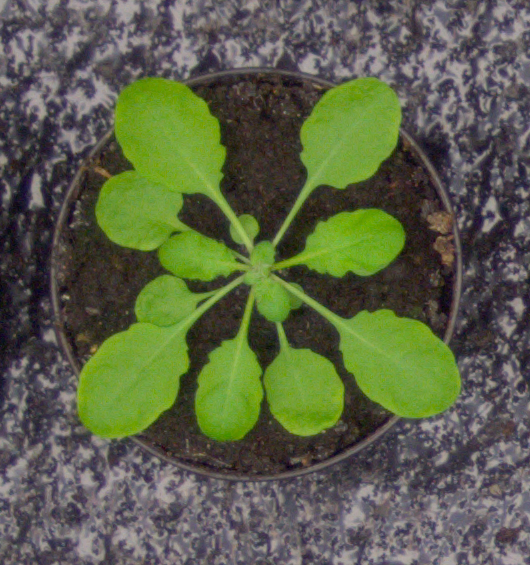
\includegraphics[width=.3\textwidth]{pic/27_rgb}}
	\qquad
	\subfloat[Classification]{
\includegraphics[width=.3\textwidth]{pic/27_class}}
	\qquad
	\subfloat[Watershed]{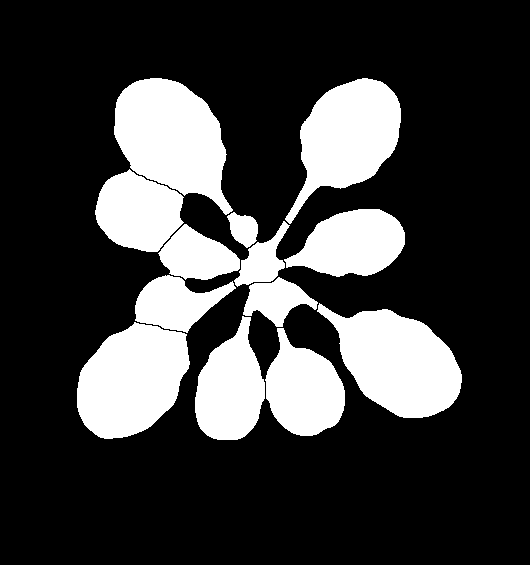
\includegraphics[width=.3\textwidth]{pic/27_watershed}}
	\qquad
	\subfloat[Particle Analysis]{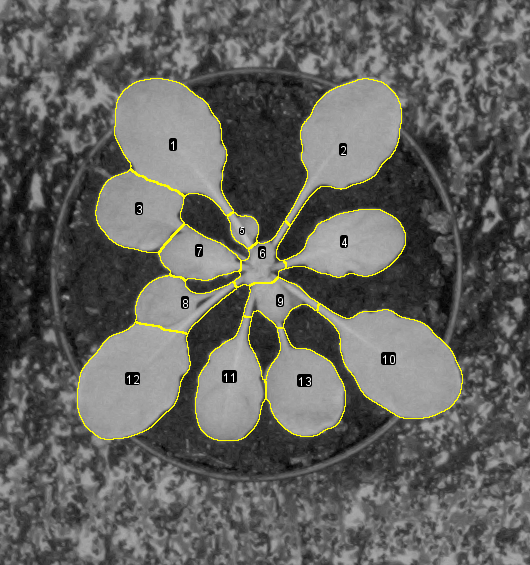
\includegraphics[width=.3\textwidth]{pic/27_greenPA}}
	\caption[Image analysis pipeline]{The analysis of plant leaves is conducted in three steps. The RGB input image (a) is classified into plant and background by a trainable Weka segmentation classifier (b). Single leaf objects are identified by watershed segmentation (c). The binary mask is used to analyze properties in the split red, green and blue channel (d).}
	\label{fig:pipeline}
\end{figure}

\subsection{Segmentation}
The plant is separated from the background with the help of a trainable Weka segmentation classifier \citep{ArgandaCarreras.2017}. Weka provides a GUI to train machine learning algorithms to produce pixel-based segmentations. The user can add traces to classes and train the classifier with those. Afterwards, traces/regions of interest can be adjusted and the classifier can be re-trained to improve classification. Six representative pictures are selected from the 2017 data set for training (plant029, plant145 and plant159 from A1; plant032, plant034 and plant037 from A2). Pictures are chosen to cover the whole range of plant green shades and the range of background characteristics of the given data sets. The Weka Experimenter was used to assess the performance of different machine learning algorithms. Based on these results (table \ref{tab:weka}), FastRandomForest was used with default parameters as a classifier. By applying the trained classifier to the RGB input images, for each input image a binary classification image is obtained (figure \ref{fig:pipeline}-b). 

\begin{table}[htbp]
	\centering
	\caption{Comparison of classifier performance by Weka Experimenter. The default algorithm parameters were kept.}
	\begin{tabular}{lllllll}
		\toprule
		Algorithm & Percent correct & Precision & Recall & F score & Matthews  & AUC \\
		 & & & & & correlation & \\
		 \midrule
		FastRandomForest & 99.93 & 1.00 & 1.00 & 1.00 & 1.00 & 1.00 \\
		SMO & 92.52 & 0.89 & 0.93 & 0.91 & 0.85 & 0.93 \\
		$k$-nearest Neighbors & 95.38 & 0.95 & 0.93 & 0.94 & 0.90 & 0.95 \\
		RandomSubSpace & 99.85 & 1.00 & 1.00 & 1.00 & 1.00 & 1.00 \\
		Bagging & 99.77 & 1.00 & 1.00 & 1.00 & 1.00 & 1.00 \\
		DesicisonTable & 99.05 & 0.99 & 0.9 & 0.99 & 0.98 & 1.00 \\
		\bottomrule
	\end{tabular}
	\label{tab:weka}
\end{table}

\subsection{Objects recognition}
A plant consists of leaves that are attached to each other. To be able to analyze leaves individually, they need to be separated. Here, the watershed algorithm was used to separate touching objects. Its implementation in Fiji is based on the algorithm described by \citet{Kunt.1990}. The algorithm first calculates an Euclidean distance map and determines center points as points which are, from a topological view, the ultimate eroded points, As the algorithm's name indicates, this topological map is "flooded" with water and at each collision of two "watersheds", a line separating two objects is drawn. Before watershed was applied, outliers were removed in both classes of the binary image by using the Fiji remove outliers function separately on each class. This function uses a median filter, for which the pixel radius was set to 6 and the threshold was set to 50. The output of the watershed algorithm is the binary image with added watershed lines (figure \ref{fig:pipeline}-c). 

\subsection{Object analysis}
After an image was subjected to the aforementioned steps, the resulting watershed image was then analyzed using Fiji's Analyze Particles tool. The measurements that were selected to be performed during the particle analysis are:

\begin{compactitem}
\item Area - Measures the area of selection in square pixels. This was used to obtain the object's size.
\item Mean gray value - Average gray value of the selection.
\item Centroid - Provides the center point of the selection as the average X and Y coordinates for all pixels in the selection or image.
\item Bounding rectangle - This is the smallest possible rectangle that encloses the selection. It gives the X and Y coordinates in respect of the upper left corner of the rectangle, as well as the height and width, from which the width-to-height-ratio will be calculated.
\item Shape descriptors - These descriptors are used to attain the roundness of each object.
\item Feret's diameter - Can be used to find the longest distance between any two points on the selection boundary.
\item Integrated density- Used to indicate the sum of the brightness, as it sums the values of the pixels in the image or selection.
\end{compactitem} 

Particles with a pixel size less than 70 were excluded from the "Analyze Particles" command. The value of 70 was established by trial and error, by inspecting the lines drawn by the watershed algorithm to separate objects.

Fiji automatically generates a Results Table, with the selected measurements. These results can be accessed by using the \texttt{getResultsTable()} method in the source code, to select the appropriate results for further use. By using this method, a csv file with all the results deemed necessary was created. 

The generated Results Table results ("columns") that were included in the csv file can be seen in Table \ref{tab:result_table}.

\begin{table}[htbp]
	\centering
	\caption{Measurement options and the corresponding value in the csv file.}
	\begin{tabular}{lll}
		\toprule
		Measurement option  & Corresponding value in the csv file \\
		\midrule
		 Display Labels & objectID and imageID\\
		Area & size\\
		Centroid & pos\_x and pos\_y\\
		Shape descriptors & roundness\\
        Integrated density & brightness\_sum\\
      	Mean gray value & brightness\_average\\
       	Bounding rectangle & width\_to\_height\_ratio\\
        \bottomrule
	\end{tabular}
	\label{tab:result_table}
\end{table}

As brightness values calculated from binary watershed images is insufficient for plants, Fiji's "Analyze Particles" command was also applied to the original RGB images. The Particle Analyzer however, can only work with one channel (ie. grayscale) images. Working with the original RGB images required a split in the color channels. The analysis was then done on the chosen channel. The brightness (both the sum and the average) of each of the three color channels (red, green and blue) were individually calculated. These individual channel results were then added together to calculate the sum of the brightness and average brightness for each object. To ensure computational efficiency not all the measurements were selected again, as this would have resulted in the duplication of results, eg. the size of the objects will remain constant, it is independent of the type of input image. The measurements that were necessary to be applied to the original RGB images, are the mean gray value and the integrated density. Results regarding the brightness of each color channel were attained and added to the csv file. 

An additional requirement of the project was to include the width to height ratio. As this is not a built-in measurement option in Fiji, the width and the height that were included in the Results Table, as part of the "Bounding rectangle" measurement were extracted and the ratio was calculated, by dividing the leaf width by the leaf height. The calculated width to height ratio was added to the csv file to be available for further use.

The Feret Ratio was additionally calculated from the minimum caliper diameter (MinFeret) and the maximum caliper (MaxFeret) values. These values are calculated as part of the Feret's diameter measurements. The ratio was calculated, by dividing MinFeret by MaxFeret, as another approach to get a width to height ratio overview for each leaf.

\subsection{Explorative data analysis}
Data analysis was conducted in Jupyter Notebooks using several Python packages. Data were handled with the python package pandas. For visual statistical analysis, the seaborn package was used. Numerical statistical analysis was mainly performed using the stats module from the python package scipy. For general plotting of graphs, the pyplot module from the python package matplotlib was used.

\subsection{Data}
For this study, datasets of the Leaf Segmentation and Counting Challenges were used \citep{Minervini.2016}. The imaging data were manually annotated to provide ground truth information \citep{Scharr.2014}. The datasets contain images of greenhouse images with \textit{A.~thaliana} and \textit{N.~tabacum}. \textit{A.~thaliana} is a rosette plant, with the individual leaves being on separate, distinguishable stems. This characteristic of \textit{A.~thaliana} makes leaf separation from each other less complex.  Given that we were only exploring viable methods in this research area, \textit{A.~thaliana} was our chosen plant, as it gave us the opportunity to explore with different algorithms in an easier way than what the \textit{N.~tabacum} dataset would have allowed us to do. Since the datasets for 2014, 2015 and 2017 are nearly the same, only differing in the amount of provided meta data, datasets from a single year were used for analysis. 

\section{Results}
\subsection{Comparison of leaf count to ground truth for the A1 and A2 datasets}
The rgb images from datasets A1 and A2 were analyzed with the previously described pipeline. Using tabular ground truth data supplied with the raw images, the output leaf count per plant was compared to the ground truth. The difference between ground truth and count was plotted for each image (figure \ref{fig:truth}). The largest difference in A1 were -21 leaves and in A2 6 leaves. For dataset A2, a root mean squared error of 2.74 was achieved, while for dataset A1, the error was 6.72. Since the results for the A1 dataset exhibited a huge deviation from ground truth, all further analyses were only done with the results from the A2 dataset.

\begin{figure}[h!]
	\subfloat[A1 Dataset]{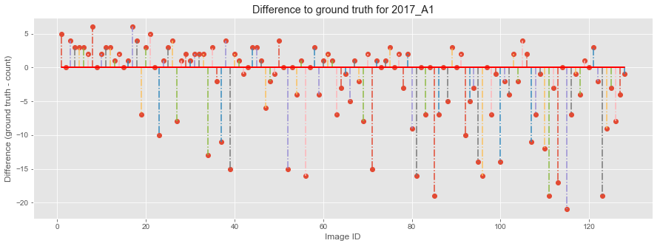
\includegraphics[scale=.6]{pic/A1-truth}}
	\qquad
	\subfloat[A2 Dataset]{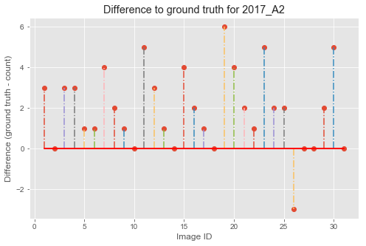
\includegraphics[scale=.5]{pic/A2-truth}}
	\caption{Comparison of the leaf count to ground truth. The ground truth was determined by manually annotation of images \citep{Scharr.2014}. The output of this approach for every single image was subtracted from the ground truth and plotted.}
	\label{fig:truth}
\end{figure}

\subsection{Overview of the A2 dataset}
To identify pairwise correlations between variables, a scatterplot matrix was plotted for the variables plant size, leaf roundness, average green brightness, feret ratio, and width to height ratio. Visual inspection indicated a linear correlation between roundness and feret ratio. 
 
\begin{figure}[h]
	\centering
	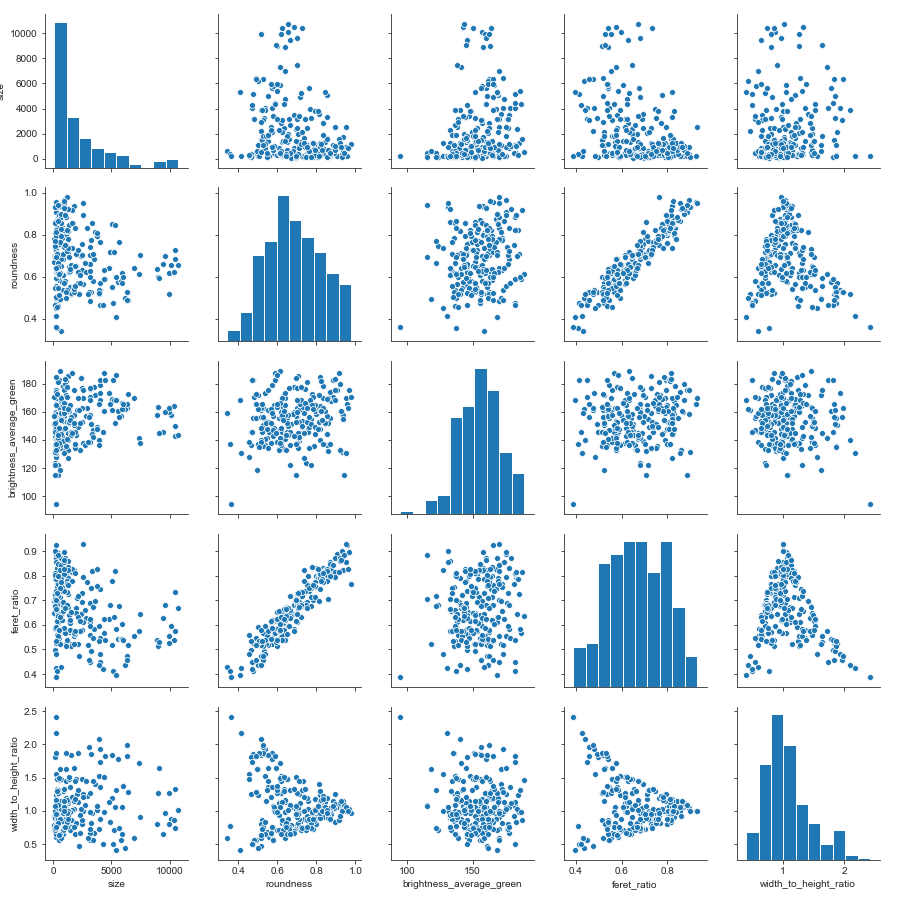
\includegraphics[width=13cm]{pic/overview}
	\caption{Overview of pairwise correlations between the features size, roundness, average green brightness, feret-ratio, and width-to-height-ratio in the 2014 datasets shown in a pairplot matrix.}
	\label{fig:overview}
\end{figure}

\subsection{Analyses of correlations}
Computation of Pearson correlation coefficients for several variables reinforced the previous visual inspection. Low correlation between size and roundness (pearson -0.23), and between size and color (pearson 0.18) were found (figure \ref{fig:corr}-A and -B). By contrast, the number of leaves correlated highly with the total plant area (pearson 0.86, \ref{fig:corr}-C). In particular, this correlation is not linear, but appears perhaps quadratic. Therefore, Spearman's rank correlation coefficient was calculated and the result was 0.94, indicating a high correlation. 

\begin{figure}[h!]
	\centering
	\subfloat[Size vs. Roundness]{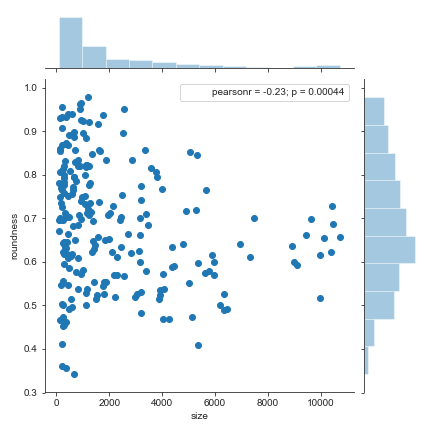
\includegraphics[width=.45\textwidth]{pic/size-roundness}}
	\qquad
	\subfloat[Size vs. Color]{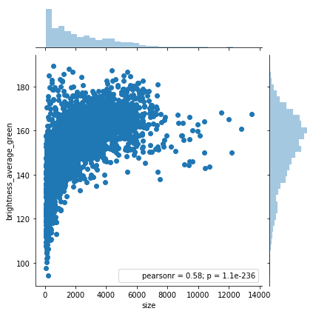
\includegraphics[width=.45\textwidth]{pic/size-color}}
	\qquad
	\subfloat[Number of Leaves vs. Total Area]{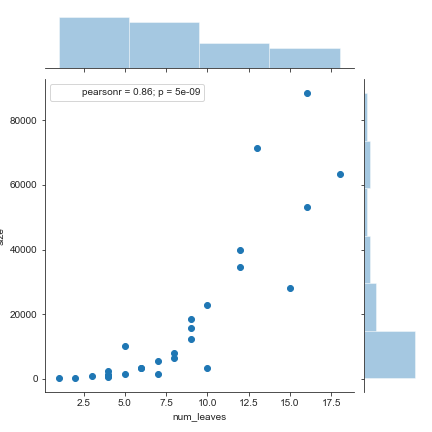
\includegraphics[width=.45\textwidth]{pic/number-area}}
	\caption{Analyses of correlations shown in pairwise scatter plots with histograms along the x- and y-axes and Pearson correlation coefficients.}
	\label{fig:corr}
\end{figure}

\section{Discussion}
\subsection{Challenges in the identification of plants}
In the pipeline suggested here, the image was first segmented into plant and background using a trainable WEKA segmentation. The quality of the classification was depending on two parameters: the selection of images and the number of images and amount of pixel traces used for training. The more images and the more pixels used for training of the classifier, the larger will be the file size and the longer it will take to read in the file and to apply the classifier to images. Thus, a balance was required between number of labeled pixels and classification accuracy because with increasing number of labeled pixels the execution of the program requires more time. A compromise between a sufficient training subset and a reasonable file size was found by using six images (three of each dataset). In general, a diverse subset of images should be selected for training. During implementation, several subsets were considered. First, the training set contained an image with a mossy plant pot and the classifier was trained to recognize moss as background. It was not possible to successfully train the classifier with that training set. Either the moss was still recognized as plant or the moss was recognized as background but also substantial parts of plants were classified as background. Therefore, it was decided to focus on a sufficiently well classification of plants and the classifier was trained with a subset that contained images with red and black background, with or without water, with red marker tape, with small and big plants and with overlapping neighboring plants but not with moss.

In this pipeline, outliers were removed using a median filter with a radius of 6 pixels. With this approach, outliers were successfully removed but the A2 dataset also contained some very small plants that got lost in this step. 

\subsection{Object Analysis}
Object analysis to be included in the generated Results Table are clearly formulated in the ImageJ documentation \citep{Ferreira.2012}. A decision that was needed to be made, was whether to take an object's position from the the top left appearing pixel or from the centroid. In this project we used the centroid to indicate the object's position, as by using the top left appearing pixel position has no advantage over the centroid. By using the centroid positions, we ensured that the position coordinates are more robust to possible rotations. If the top left appearing pixel was used, problems could arrive if the leaves were to be rotated. 

In  the Fiji Results Table, circularity and roundness are two similar measurements. Circularity in ImageJ is calculated in such a way that it excludes local irregularities, therefore the roundness measurement, which gives a value directly relative to the aspect ratio, was included in the csv file. 

After calculating both the width to height ratio and the Feret ratio for each leaf, it was found that although the two ratio's did render corresponding values in some instances, there were other instances where the ratio values differed significantly. Manual calculations were done (measuring the length and width of a leaf on-screen with a ruler) and it was found that in the cases where there was a difference between the ratios, the Feret ratio was more accurate. The reason is that the bounding rectangle is not turned by Fiji according to the leaf's position, instead the bounding rectangle remains parallel to the image border and is thus in certain cases a rough estimate of the approximate height and width. As previously discussed in the methodology section, the Feret's ratio is calculated from exact measurements and therefore leads to more precise results. 

\subsection{Quality of the analysis of the A1 dataset}
The analysis of the A1 dataset showed a huge deviation of number of objects from the ground truth. The largest difference was -21 leaves, so the program identified a lot more as leaves than the image contained. To identify the reason for the misclassification, the output images were visually compared on a sample basis to the ground truth images. Considering the ground truth images, it was found out that mainly mossy parts of plant pots were misidentified as plant area although moss should be identified as background. This can be attributed to the choice of classifier in the first step of the pipeline. It appeared that the used Weka segmentation based mainly on the color of the pixels. The datasets contained plant images with various shades of green. Therefore, the classifier was not able to distinguish bright pixels belonging to plant from bright pixels belonging to moss. A negative classification example can be found in figure \ref{fig:moss}. The lower left quarter of the plant pot did not contain a leave but most of this area was classified as plant. 
To prevent the misclassification of mossy plant pots, a different approach could be tested, e.g. convolutional neural networks. The above described approach could be improved by taking other features, like granularity, into account.

\begin{figure}
	\centering
	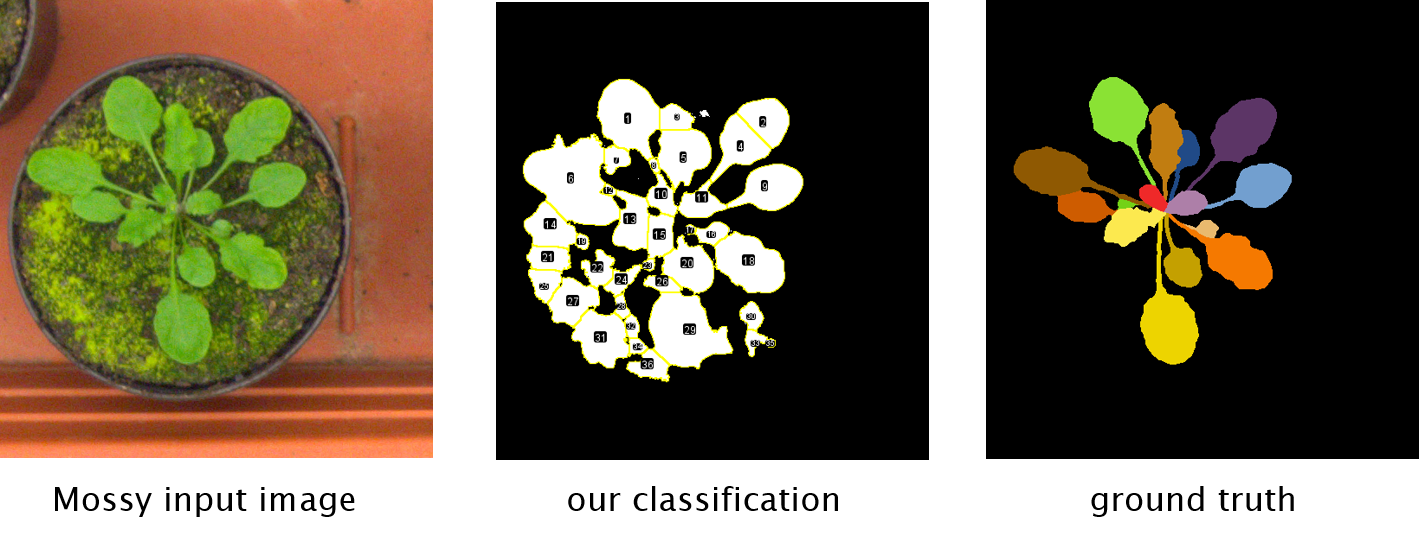
\includegraphics[width=13cm]{pic/moss}
	\caption{Example of the classification of a mossy plant pot in comparison to ground truth. The moss was mainly incorrectly classified as plant.}
	\label{fig:moss}
\end{figure}

\subsection{Correlations in leaf characteristics}
The determined leaf characteristics were analyzed regarding correlations between pairwise measures. A high correlation between roundness and feret radio was found. This is unsurprising, since each feature measures object roundness, albeit in different ways. 

In addition, a high, non-linear correlation between number of leaves and total plant area was shown in the data. This aligns with prior biological knowledge: a plant tends to sprout many small leaves early, which then grow in area over time.

\section{Conclusion}
The project's goal was met in that we did successfully implement a simple and naïve approach towards plant classification by using top view photos. By applying Trainable Weka Segmentation, with a FastRandomForest classifier, a plant was separated from its background in simple cases. Leaf separation and subsequent analysis of individual leaves were carried out successfully. 

Through the application of various statistical functions in-depth analysis were performed and it was found that the FastRandomForest classifier (used with standard Fiji settings) was not able to successfully distinguish between leaves belonging to the plant and moss surrounding the plants. We concluded that this inabillity of the classifier was due the classifier basing classification mostly on color. 

To improve the performance of our classifier on the A1, mossy, dataset we suggest to in future make use of different hyperparameters, that can for example differentiate based on coarseness, as plant leaves have smoother appearance than moss. More detailed and sensible preprocessing to distinguish the moss as noise can be another viable option to consider in order to improve the classifier's accuracy.


\renewcommand\bibname{References} % necessarily before \bibliography{ref}, but not working in preamble
\bibliographystyle{apalike} % for references chapter
\bibliography{ref}

\end{document}
